\documentclass[%
 reprint,
%superscriptaddress,
%groupedaddress,
%unsortedaddress,
%runinaddress,
%frontmatterverbose, 
%preprint,
%preprintnumbers,
nofootinbib,
%nobibnotes,
%bibnotes,
 amsmath,amssymb,
 aps,
%pra,
%prb,
%rmp,
%prstab,
%prstper,
%floatfix,
]{revtex4-2}

\usepackage{MyResources}

\begin{document}



\title{An Introduction to Quantum Kernel Estimation}% Force line breaks with \\


\author{Joseph Merritt}

\begin{abstract}
The fields of Machine Learning (ML) and Quantum Computing (QC) have made strong advances in recent years. Each is often associated with one or more seminal problems that the technology excels at solving, and these problems usually do not overlap. It might seem surprising, then, that these two technologies would have something to offer one another. Recent proposals have been made that would allow quantum computing to have an advantage over classical computing in certain machine learning tasks. One such proposal is known as Quantum Kernel Estimation (QKE). This article introduces QKE and gives a brief overview of topics in ML and QC.
\end{abstract}

\date{\today}% It is always \today, today,
             %  but any date may be explicitly specified

%\keywords{Suggested keywords}%Use showkeys class option if keyword
                              %display desired
\maketitle
% \maketitle needs to come after the abstract and stuff

%\tableofcontents

\section{Introduction}
In recent years, significant attention has been given to the field of Machine Learning (ML). Machine learning has been used in a variety of contexts to solve difficult computational problems, such as pattern recognition and data classification.

One major area of machine learning is \textit{binary classification}. In a binary classification problem, a given input must be classified into one of two categories.
%For example, consider the problem of determining whether a traffic light is red or green based on an image of the traffic light. Without machine learning, this problem would be solved manually by first identifying patterns that are consistent between all images of red lights and green lights and then programming an algorithm to check for these patterns. 
%Such an algorithm might contain the following steps:
%Such an algorithm--a series of steps taken to solve a problem, often involving mathematics--might contain the following steps:
\begin{comment}
\begin{enumerate}

\item Use edge detection to find the three circles indicating the boundaries of three lights (red, yellow, green).

\item Use the circles' positions to determine which circles correspond to the red and green lights.

\item Calculate the average color inside the circles corresponding to the red and green lights.

\item Compare the average colors to each other to determine which light is more likely to be lit.

\end{enumerate}
\end{comment}
For large or complex sets of data, this can be very difficult to solve. 
For instance, imagine a program that could differentiate images of cats from images of dogs. It would be extremely difficult to identify a list of features that a program could use to distinguish these images, especially given the many shapes, sizes, and colors of dogs and cats.
For classification problems such as these, machine learning was developed. 
%In the given machine learning problem of differentiating dog images from cat images, 
In machine learning, the key characteristics used to discriminate between the two categories are not programmed manually. Rather, the program is designed to ``learn'' the key distinguishing characteristics. This is done by making a program that can accept training data (i.e., images that are already known to be of either a dog or a cat) and use these data to determine a ``boundary'' between cat images and dog images. This boundary can be used to classify images that are not in the training data by determining which side of the boundary contains the image.

Such machine learning approaches have been used in a variety of areas with great success, including image, text, and speech recognition; language translation; image and text generation; and data analysis and prediction.

Another recent technology receiving great attention is quantum computing. Quantum computing attempts to use quantum physics--which describes very small objects, usually at very low temperatures--to solve computational problems. This is contrasted with the common ``classical'' computing paradigm, in which electrical physics (e.g., an electronic circuit) is used to solve computational problems.

While many claims have been made about quantum computing, it is not expected to have complete superiority over classical computing. It is expected that 
%both classical and quantum computing will 
certain problems will be less expensive (in terms of time and physical resources) to solve using classical computers, and the optimal solution to many problems will involve a combination of both classical and quantum computing resources. Quantum computers are not simply faster versions of classical computers, but instead perform computations in a fundamentally different way, owing to the unique nature of quantum physics. 
%Thus, it is expected that many specific problems are more efficiently solved by quantum computing.

%Two broad types of quantum computing are in use today: circuit-based quantum computing, and quantum annealing. For this article, we will ignore quantum annealing and consider only to circuit-based quantum computing.

Many theorized applications of quantum computers are for research purposes. Early proposals focused on using quantum computers as a natural framework for simulating quantum systems. This extends to research in particle physics, materials science, and drug discovery. However, information-focused applications have been proposed as well. An early seminal result described a quantum algorithm that can quickly find the factors of a large number. 
That is, given only a large number which is the product of two prime numbers, the proposed quantum algorithm determines the two prime numbers of which it is a product and performs this task more quickly\footnote{A more technical statement of the algorithm's speed advantage is the following: for any classical algorithm that factors a number into its two prime factors, there is a ``critical'' number such that the quantum algorithm will outperform the classical algorithm when factoring numbers larger than this critical number.} than any known classical computing algorithm \cite{shor_polynomial-time_1997}. If such a quantum algorithm could be efficiently executed on quantum hardware, it would undermine the foundation of RSA encryption used for internet security, as the encryption technique relies heavily on the computational difficulty of factoring large numbers.

Current efforts in quantum computing are mainly focused on improving quantum hardware. Primary areas of interest include increasing the amount of available quantum resources per computer, increasing the speed of quantum operations, and decreasing noise and hardware errors.

Despite the apparent dissimilarity between the fields of machine learning and quantum computing, advantages in their combined use have been proposed. These integrations can be broadly separated into two categories: machine learning improving quantum computing (such as using ML to assist in simulating quantum hardware), and quantum computing improving machine learning. This article will focus on the latter case. In particular, a method will be introduced in which quantum computing can enhance Support Vector Machine training by using Quantum Kernel Estimation \cite{noauthor_seeking_2023, russo_quantum_2023}.

An overview of machine learning is given in Sec. \ref{sec:ML}, with particular emphasis on Support Vector Machines (SVM). An introduction to the fundamentals of quantum computing is given in Sec. \ref{sec:QC}, with emphasis on the vector nature of quantum states. Finally, an example in which quantum computing can boost the efficiency of machine learning is given in Sec. \ref{sec:QML}.

\section{Machine Learning}
\label{sec:ML}

Computers have become universal across every aspect of modern life. As computers have become more powerful, it has allowed new areas in computer science to flourish. One such area is Machine Learning (ML). It is primarily concerned with the design and operation of programs, called models, that solve a problem by ``learning'' the solution from data rather than by being directly programmed to solve a problem.

As stated before, an important area of ML is the study of \textit{binary classification} problems, where input must be classified into one of two categories. One approach to solving a binary classification problem is to create a Support Vector Machine (SVM), which is a type of machine learning model designed specifically for solving classification problems. This section will cover information regarding SVMs and the theory behind their operation.

\subsection{Support Vector Machines}

A Support Vector Machine is a model that classifies input into one of two categories. To more precisely describe how such a model works, the following example problem will be considered: two types of flowers, roses and dahlias, are to be distinguished based on two characteristics, the number of petals and the (average) petal length in centimeters. A model that solves this problem will be able to accurately classify a flower as a rose or a dahlia based on the number of petals a flower has and the length of those petals.

The first step in creating this model is to collect a large data set containing data for roses and dahlias. This is called the \textit{training data set}. The training data set is collected and categorized by humans before the model is created. Each element in the set will contain two entries: a \textit{label} and a \textit{vector}. The label classifies each flower as a rose or dahlia and is supplied by a human who manually categorizes each flower. A \textit{vector} is by definition a list of numbers. The vector of a training data set element is a list of two numbers: the number of petals and petal length in centimeters. The dimension of a vector is the number of numbers used to define the vector. Therefore, each element of the training data set contains a label and a two-dimensional vector.

A fictitious example of such training data is graphed in Fig. \ref{fig:2d_noline}, with the number of petals on the horizontal axis and petal length on the vertical axis. Each point is a two-dimensional vector representing the data of one flower.

\begin{figure}
    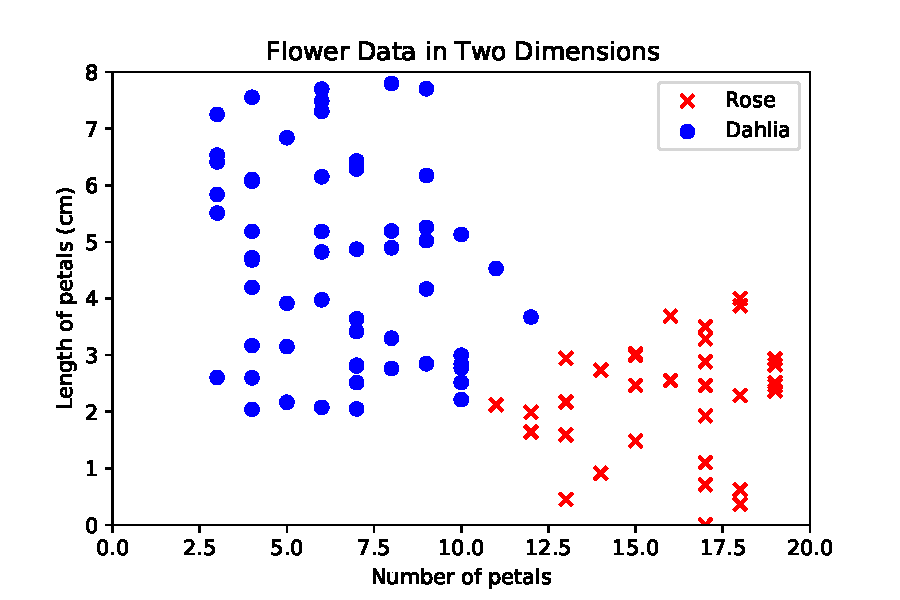
\includegraphics[width=\linewidth]{Figures/2d_noline.pdf}
    \caption{\label{fig:2d_noline}A scatterplot of training data \cite{noauthor_all_nodate}. Each point is a vector, defined by two numbers: the number of petals (on the horizontal axis) and the length of the petals in centimeters (on the vertical axis). The label identifies each flower as a rose or dahlia. The data is fictitious and used only for explanatory purposes.}
\end{figure}

\begin{figure}
    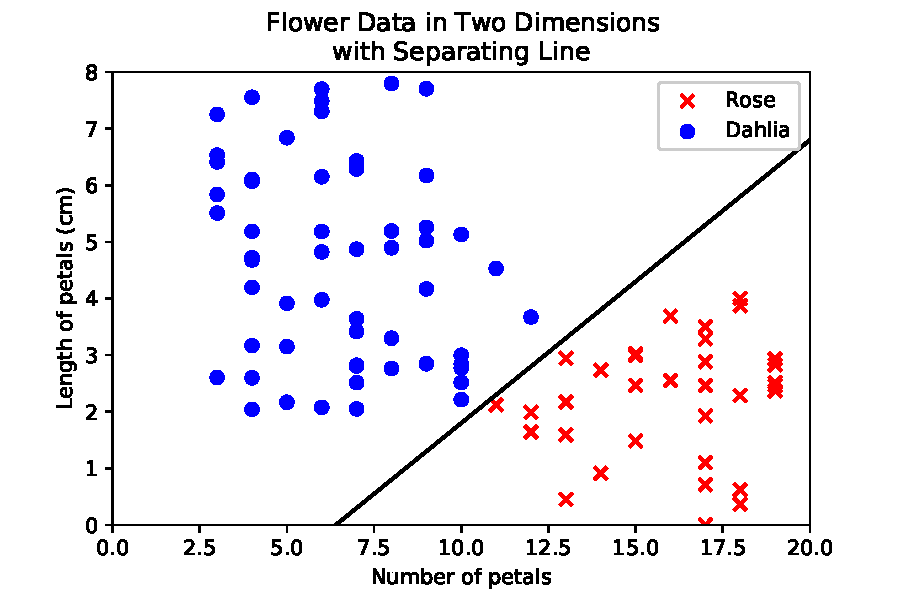
\includegraphics[width=\linewidth]{Figures/2d_line.pdf}
    \caption{\label{fig:2d_line}One possible way to separate the training data of Fig. \ref{fig:2d_noline} with a line. This line perfectly separates the data and proves the data is \textit{linearly separable}. Note that this line is not the optimal line that would be found by a Support Vector Machine.}
\end{figure}

The second step in creating such a model is to \textit{train} the model using the training data. This means separating the data in Fig. \ref{fig:2d_noline} into a ``rose region'' and a ``dahlia region''. 
%Examples of such separations are shown in Fig. \ref{fig:2d_line}.
A Support Vector Machine separates the training data using a straight line called a \textit{separating line}. An example is shown in Fig. \ref{fig:2d_line}. A line is chosen which satisfies certain equations and results in an optimal line. The location of the optimal line is determined by the so-called \textit{support vectors}, which are the vectors closest to the separating line. Once a separating line has been found, the SVM can now classify new data that was not part of the training data. It does this by using the separating line to determine if a new data vector is in the rose region or the dahlia region defined by the separating line.

If the training data can be separated perfectly by a line, such that all data from one category are on one side of the line and all data from the second category are on the other, then the training data are said to be \textit{linearly separable}. If the training data are linearly separable, then the optimal separating line found by the SVM will be the same distance from the nearest data in both categories. That is, the shortest distance between the line and any data in the first category is the same as the shortest distance between the line and any data in the second category.

It is common to find that the training data are not linearly separable. Take, for example, the training data graphed in Fig. \ref{fig:3d_line}. In this case, no line cleanly separates all roses from dahlias. An optimal line can still be found, but this will mischaracterize some training data, and some roses will be classified as dahlias and vice versa. Alternatively, one could add another dimension to the data. For example, petal width can be measured in addition to the number of petals and petal size. Each flower is then described by a three-dimensional vector. Adding this new dimension to the data in Fig. \ref{fig:3d_line} could result in a data distribution such as that in Fig. \ref{fig:3d_noplane}.

\begin{figure}
    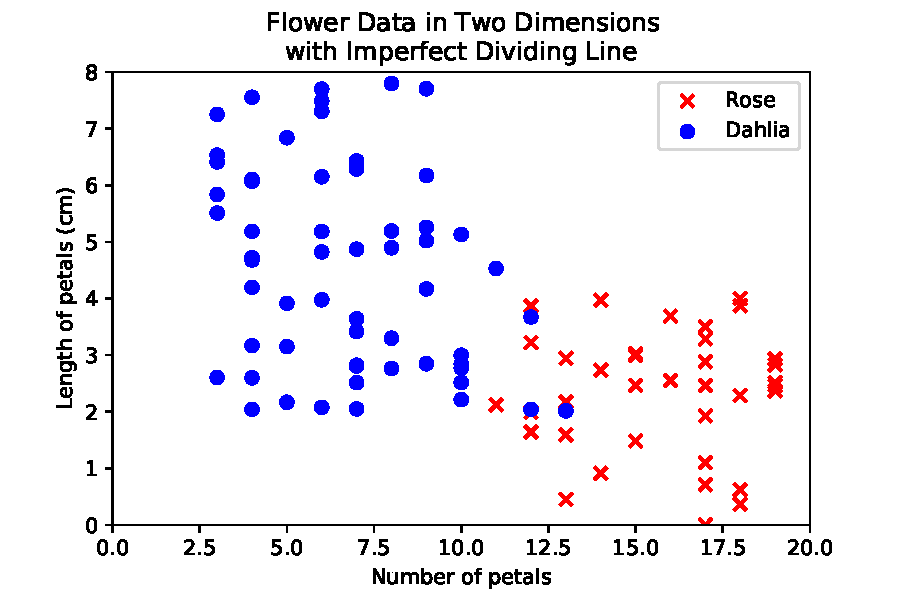
\includegraphics[width=\linewidth]{Figures/3d_line.pdf}
    \caption{\label{fig:3d_line}An example of data that is not linearly separable. As a result, no line gives a perfect separation of the training data; every line will have data from both categories on either side.}
\end{figure}

\begin{figure}
    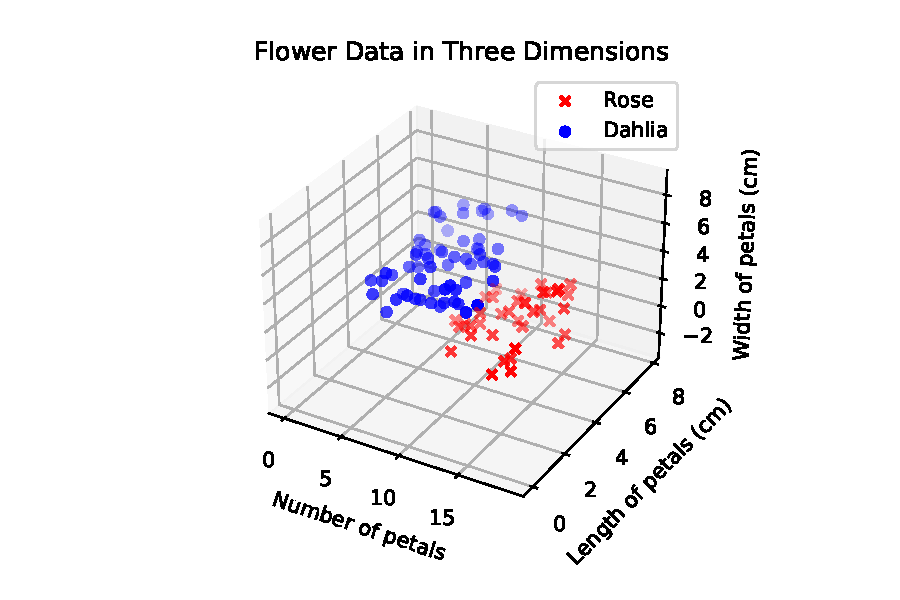
\includegraphics[width=\linewidth]{Figures/3d_noplane.pdf}
    \caption{\label{fig:3d_noplane}An example of a training data set with three-dimensional vectors \cite{noauthor_all_nodate}. Each point is a vector, defined by three numbers: the number of petals, the length of the petals in centimeters, and the width of the petals in centimeters. The label identifies each flower as a rose or dahlia. Ignoring the vertical axis, the positions of the vectors along the two horizontal axes are identical to the data in Fig. \ref{fig:3d_line}. This data is fictitious and used only for explanatory purposes.}
\end{figure}

When working with three-dimensional vectors of data, the goal of an SVM is now to find the optimal plane that separates the two categories of data. An example of a \textit{separating plane} is shown in Fig. \ref{fig:3d_plane}. The key insight is that these data, while unable to be separated using two dimensions, can be perfectly separated using the additional dimension.

If the training data can be perfectly separated by a plane, then the data is said to be linearly separable, as in the two-dimensional case.

\begin{figure}
    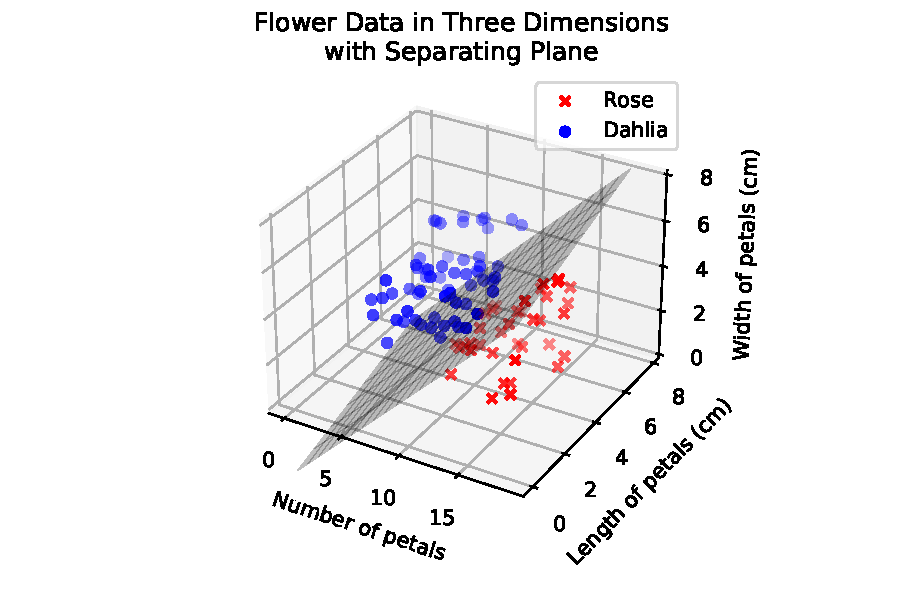
\includegraphics[width=\linewidth]{Figures/3d_plane.pdf}
    \caption{\label{fig:3d_plane}One possible way to separate the three-dimensional training data of Fig. \ref{fig:3d_noplane} with a plane. This plane perfectly separates the data and proves the data is \textit{linearly separable}. Note that this plane is not the optimal plane that would be found by a Support Vector Machine.}
\end{figure}

This can be continued by adding different types of flower measurements to the training data set, which may be required to accurately distinguish flowers using real data. In higher dimensions, the goal of an SVM is to find an optimal separating ``hyperplane'' which separates the training data into its categories. If such a hyperplane can be found that perfectly separates the data, the data are said to be linearly separable, regardless of the number of dimensions.

There is a computational cost associated with adding dimensions to a data set. When there are more numbers in a data set, a computer must perform more calculations to find the separating hyperplane. This will require more computational resources--more energy, memory, and time.

This highlights an important trade-off in training SVMs (and other ML models in general). Generally, it will be easier for a model to categorize data when the data have a higher number of dimensions. However, increasing the number of dimensions also increases the difficulty of training the model.

To give some examples, note that for certain speech-generating models, each word is mapped to a unique dimension. For instance, a model that knows 10,000 words might represent a word as a 10,000-dimensional vector--a list of 10,000 numbers--where each number represents a single word. For image recognition models, an image with a size of 256-by-256 pixels includes three color values (red, green, and blue) for each pixel. This means each image is defined by a list of nearly 200,000 numbers--a 200,000-dimensional vector. 

Furthermore, models are generally more accurate when the training data contains many examples, which also increases the difficulty of the calculation. An SVM trained using 1,000 images, each of which has a size of 256x256 pixels, would need to perform calculations on nearly 200 million numbers to complete its training. In practice, high-quality models require far more data than this. Therefore, the high number of calculations that must be performed becomes a major challenge when training machine learning models.

\subsection{Kernel Function SVMs}

Due to the computational difficulty in training models, methods have been proposed that attempt to increase the efficiency of training. One of these methods, which involves the use of a function called a \textit{kernel}, will now be described.

The SVM introduced in the previous subsection is known as a \textit{linear} SVM\footnote{This is because the separating hyperplane found by training the SVM is the solution to a linear set of equations.}. 
%In contrast, there are training data sets where a clean categorization cannot be accomplished with a separating hyperplane.
For certain data sets, a hyperplane may not be the best way to distinguish categories of data.
Instead, a more complicated surface may be better suited as the boundary between categories. Nevertheless, an arbitrarily complex surface with a high number of dimensions can be very difficult to describe. It would then be advantageous to find a relatively simple way to describe a complex surface amenable for use in an SVM.

Training data that are not linearly separable might become linearly separable when more dimensions are added. One way of doing this is to add another dimension of data to the elements in the training data set, as described previously. Another way of adding dimensions is to map the data to higher-dimensional vectors. This can be done by choosing a function that, when given a vector, returns a vector with a higher number of dimensions. When applied to training data, the data are said to be mapped to a higher-dimensional vector by the function. The specific function used for this would be chosen based on the nature of the problem being solved and the properties of the training data. The function will generally be different for different problems.

Fig. \ref{fig:kern_2d} shows an example of two-dimensional training data that are not linearly separable. Fig. \ref{fig:kern_3d} shows the same data, now mapped to three-dimensional vectors by the function $z = |x| + |y|$. That is, the ``height'' of each point is equal to the sum of the absolute values of the two original values of the two-dimensional vector. The new three-dimensional data vectors are linearly separable, with the separating plane shown in Fig. \ref{fig:kern_3d}.

\begin{figure}
    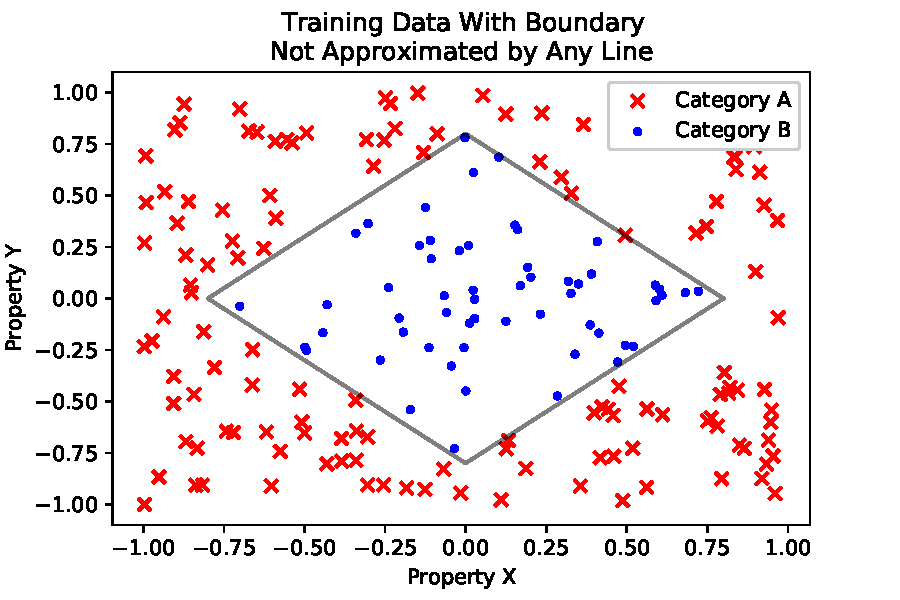
\includegraphics[width=\linewidth]{Figures/kern_2d.pdf}
    \caption{\label{fig:kern_2d}A set of training data that cannot be linearly separated. However, under the mapping $(x,y) \rightarrow (x,y, |x|+|y|)$, the results of which are shown in Fig. \ref{fig:kern_3d}, the data \textit{is} linearly separable. The plane shown in Fig. \ref{fig:kern_3d} separates the data. The boundary shown in black is the effective boundary defined by the plane when viewed in the original two dimensions of the training data.}
\end{figure}

\begin{figure}
    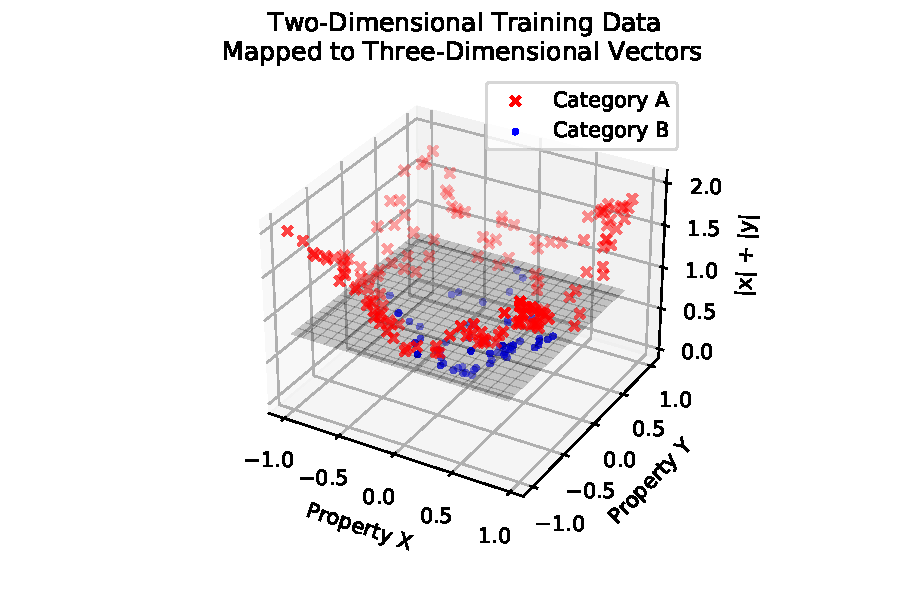
\includegraphics[width=\linewidth]{Figures/kern_3d.pdf}
    \caption{\label{fig:kern_3d}The training data shown in Fig. \ref{fig:kern_2d} after applying the mapping $(x,y) \rightarrow (x,y,|x|+|y|)$. These higher-dimensional vectors are linearly separable. This means that an SVM will be able to find the optimal separating plane.}
\end{figure}

Fig \ref{fig:kern_2d} graphs the effective boundary that the plane defines in two dimensions, which is shown to be nonlinear.
This demonstrates that the mapping allows an SVM to classify data in two dimensions using shapes more complicated than a straight line.
The difference is that now the mapped, three-dimensional data are used to train the model rather than the two-dimensional data.
%In more general settings, this method allows the mapped data to be separated by a hyperplane in a way that corresponds to a more complicated boundary in the original training data. The ability to use a mapping to effectively describe a more complicated boundary is called the ``kernel trick.''
In more general settings, this method, called the ``kernel trick,'' allows training data to be separated by a boundary that is more complicated than a hyperplane by using a hyperplane to separate a higher-dimensional version of the data to which the training data has been mapped.

In this example, the function was simple and added a single dimension. In more realistic examples the function may be much more complex and add multiple dimensions to the data. For any particular problem, a function will be chosen that is conducive to the goals of the model and accords with certain relevant properties of the data.

While the kernel trick allows a more complicated boundary between categories to be found, it requires more dimensions, and this makes it more difficult for the SVM to calculate the boundary. However, there is a way to mimic the effect of mapping the data to higher-dimensional vectors without performing the mapping. 
%This relies on a function called the \textit{kernel}.

The algorithm used by an SVM to calculate the separating hyperplane does not directly require the data vectors, but their inner products. 
The \textit{inner product} of two vectors is a particular way of multiplying two vectors together, resulting in a single number\footnote{Specifically, the inner product of two vectors in this context is equal to the product of the length of the two vectors (calculated using Pythagorean Theorem) multiplied by the cosine of the angle between them.}.
When using the kernel trick, an SVM requires the inner product of all pairs of higher-dimensional vectors that the training data are mapped to.
Sometimes a function of two vectors can be found, called a \textit{kernel}, such that when applied to two training data vectors will calculate this inner product directly. This avoids the need to perform the mapping and makes using the kernel a more efficient method for applying the kernel trick. Nevertheless, calculating the kernel of all pairs of vectors is the most computationally difficult part of using the kernel function to train an SVM \cite{russo_quantum_2023}. 

It is at this step that the possibility of a quantum advantage is highlighted. There may be a quantum program that can outperform all known classical programs when trying to solve this problem, namely, calculating the kernel values between all training data vector pairs. In the next section, the principles of quantum computing are introduced, with a focus on the concepts that will be important for using quantum computing to calculate the kernel for an SVM.

\section{Quantum Computing}
\label{sec:QC}

Quantum computing is a field of study that borrows heavily from both computer science and physics. It studies methods by which quantum physics could be used to solve computational problems.

Quantum physics (or quantum mechanics) is the study of the behavior of very small objects (often individual particles or atoms), usually at very low temperatures. In these conditions, matter and energy behave differently than they do in ``ordinary'' physics which describes the behavior of large collections of particles. In what follows, \textit{classical physics} is used to describe the behavior of the large (``macroscopic'') objects of common everyday experience.

\subsection{Classical Computing}

Almost all computing that is used today is \textit{classical computing}, implemented by electronic machines and digital circuits. The field of classical computing can be separated into two broad categories: software (programs and algorithms that are used to solve problems) and hardware (the physical machines that the programs are executed on). 

In digital computer software, the fundamental unit of data is the \textit{bit}. A bit has the defining property that it is in one of two allowed states, denoted 0 and 1. For example, the string of characters ``010'' can be said to contain three bits of information. The second bit is in the ``1'' state while the first and third bits are in the ``0'' state. These form one possible state of a string of three bits. One can check that a string of three bits can be in a total of eight possible states. A bit cannot be in any state except the 0 or 1 state, and it must always be in either the 0 or 1 state.

Any sequence of bits that are to be considered as a whole will be called a bit-string. While a single bit must be in exactly one of two states, a string of $n$ bits will be in one of $2^n$ states. The number of possible states increases exponentially as more bits are added to a bit-string. A bit-string can be represented as a number in a straightforward way: starting with 0 represented as the bit string 000, 1 is represented as 001, 2 as 010, 3 as 011, 4 as 100, and so on. Representing larger numbers requires more bits, but given enough bits, any number can be represented. Similarly, bits can be used to represent letters: A represented as 001, B as 010, C as 011, and so on. In this way, bit-strings can be used to represent (or encode) a wide variety of data.

Fundamentally, software is concerned with bit-strings and operations on bit-strings. Moreover, it includes operations in which the state of one bit-string affects an operation on another bit-string. This can be interpreted as a mathematical operation between two numbers, using the previous representation. An ordered set of operations meant to be performed on bit-strings is called an algorithm. The implementation of one or more algorithms is called a program.

By contrast, hardware is concerned with the physical implementation of bit-strings and bit-string operations in machines. In classical computing, the physics of electronic circuits is used to manipulate bit-strings. Bits are represented by the state of some electric or magnetic component in a machine. For example, a wire meant to carry one bit of information may have its voltage constrained by the machine to take one of two possible values at any time, corresponding to the two states of a bit. Electronic circuits then implement operations on bit-strings and store the results. In this way, the fundamental operations of software are implemented in the machine and the machine can be used to solve computational problems.

\subsection{Quantum circuits}

Quantum computing can be broadly separated into two paradigms: quantum circuits (described below), and quantum annealing. This article will only be focused on quantum circuits, and any references to quantum computing will implicitly refer to the quantum circuit paradigm.

The first difference between classical and quantum computing is in the fundamental unit of information. While classical computing uses a classical bit which can be in one of two states (0 or 1), quantum computing uses a quantum bit (or \textit{qubit}) which has a more complex behavior. In the same way that the behavior of a classical bit is determined by the physics of the electronic circuits used to represent it, the behavior of a qubit is determined by the quantum physics of the materials used to represent it.

\subsubsection{Electron Magnetic Moment}

To understand the behavior of a qubit, it is helpful to describe a quantum system that shares its behavior: the magnetic moment of an electron. An electron acts as a very small magnet, with a north and south pole. When the electron interacts magnetically with its surroundings--say, by being attracted or repelled by another, external, magnet--it is found experimentally that the direction of the electron's north pole always faces either toward or away from the magnet. That is to say, the electron is never seen to behave as if the north pole is facing any direction other than directly toward or directly away from the external magnet. It is said that the measurement had a \textit{result} of ``towards'' or ``away,'' depending on the subsequent behavior of the electron.

It is difficult to express how strange this is, being distinctly different from the behavior of common ``classical'' magnets that are allowed to point in any direction. This strange behavior is a fundamental part of quantum mechanics and is in fact where its name originates: the direction of the north pole is ``quantized,'' i.e., constrained to a discrete set of values (``towards'' or ``away'').

Considering this, the following is a list of significant ways in which quantum physics (e.g., the behavior of the magnetic moment of an electron) differs from classical physics (e.g., the behavior of a common bar magnet):
\begin{itemize}

    \item \textbf{Quantization:} Values describing the quantum object can be \textit{quantized}, or constrained to take certain, discrete values. For instance, an electron's north pole will always point either ``towards'' or ``away'' from a nearby bar magnet. These quantized states will be called the \textit{basis states}.

    \item \textbf{Superposition:} When the electron is \textit{not} in the presence of a magnet, the electron can be in a \textit{superposition} of the two quantized (basis) states. This is not the same as having the north pole of the electron point in a different direction, as explained in the next point below. Because of this principle of superposition, the true state of the electron is a two-dimensional vector, with a number $x$ associated with the ``towards'' state and another number $y$ associated with the ``away'' state. An interpretation of these numbers will be given shortly. It is important to understand that a quantum object with two quantum states is described by a two-dimensional vector, in contrast to a classical object with two states (e.g., a coin that is face up or face down), which only requires identifying which of the two states the classical object is in.

    \item \textbf{Wavefunction Collapse:} Although the electron can be in a superposition of basis states, when the electron is \textit{measured} (that is, placed in a situation where the value of its state determines its behavior, such as when traveling near a magnet), it will act as if it is in \textit{only one} of the basis states (i.e., with the north pole pointing either towards or away from the magnet). If the electron is in a superposition of states, its behavior will not be an average of ``towards'' and ``away'' behaviors but will follow one type of behavior precisely. Moreover, the electron will afterward no longer be in a superposition, but its state will be one of the basis states. It is as if measuring the electron forced it into one of the basis states. This phenomenon is called \textit{wavefunction collapse.}

\end{itemize}

The state of the electron after measurement is influenced by the superposition before measurement. The two values associated with each of the two basis states (``towards'' and ``away'') determine the probability that the electron will collapse onto the corresponding basis state during measurement. 
Consider an electron in the superposition state $(0.4, 0.9)$, where $0.4$ is associated with the ``toward'' basis state and $0.9$ is associated with the ``away'' basis state. A measurement of the electron (e.g., by the introduction of a magnet) is more likely to have an ``away'' result, as the number associated with that basis state is larger than that of the other basis state.
However, there is an intrinsic element of randomness, in that knowing the state of the electron (i.e., the values of the superposition) does not give enough information to predict with 100\% certainty what state the electron will be in after a measurement.
    

\subsubsection{Qubits}

The fundamental unit of information in quantum computing is the qubit. Like the electron magnetic moment, a qubit has two basis states. Instead of ``toward'' and ``away,'' these basis states will be called ``0'' and ``1'' in analogy to the classical bit. It is convention that a quantum state is written as a ``ket'' like so: $\ket{0}$, $\ket{1}$. While a classical bit must be in one of two states, a qubit can be in a superposition of two basis states, specified by a two-dimensional vector.
%, allowing for far more possibilities than one bit can allow. 
When a qubit is measured, it is not possible to recover all of the information about its true quantum state. Measurement collapses the qubit onto one of its basis states, resulting in only two possible values: 0 or 1.

This behavior continues as more qubits are used. A collection of qubits is called a \textit{quantum register}. Each basis state of the quantum register is the combination of one basis state from each qubit. For a register with three qubits, where each qubit has two basis states labeled $\ket{0}$ and $\ket{1}$, there are eight total basis states: $\ket{000}$, $\ket{001}$, $\ket{010}$, $\ket{011}$, $\ket{100}$, $\ket{101}$, $\ket{110}$, and $\ket{111}$. The quantum register can be in a superposition of these eight basis states, making the state an eight-dimensional vector. 
In general, the basis states for a quantum register of $n$ qubits are labeled by the $2^n$ possible bit-strings of $n$ bits, making the state of a quantum register a $2^n$-dimensional vector\footnote{Technically, this is a vector of $2^n$ \textit{complex} numbers, where each complex number is specified by two real numbers. Accounting for a normalized state and an ignored global phase, this means that the quantum register of $n$ qubits is defined by $4^n - 2$ numbers. Nevertheless, the number of dimensions grows exponentially with an increasing number of qubits $n$.}. As the number of qubits increases, the number of dimensions grows exponentially.

The primary components of a quantum computing calculation are as follows. First, the register is placed in a default initial state (e.g., the state $\ket{0000...}$). Then, operations are performed on the register which will, in general, change the state into a superposition. This series of operations applied to the register is called the \textit{quantum circuit}. Finally, some or all of the qubits in the register are measured, each having a result of $\ket{0}$ or $\ket{1}$. 

It might seem that there is no advantage in quantum computing if all the unique superposition information of a qubit is destroyed when measuring it. There are still ways in which the information can be used. First, recall that the vector describing the qubit determines how likely each measurement outcome ($\ket{0}$ or $\ket{1}$) is. By repeating the same circuit many times on the same initial quantum state (i.e., the state $\ket{0000..}$) and comparing the frequency of $\ket{0}$ to $\ket{1}$ results, the relative sizes of the numbers in the vector can be obtained. Furthermore, advanced quantum circuits are designed to take advantage of quantum superposition \textit{before} the qubits are measured, such that the quantum superposition, which was used during the calculation, is removed before the circuit is completed. This allows for a quantum advantage over classical circuits, even if quantum superposition is never directly measured.

%Classically, a bit-string of $n$ bits can be in one of $2^n$ states. For qubits, the basis states are described by bit-strings, and thus the state of a quantum register of $n$ qubits is a $2^n$-dimensional vector space\footnote{Technically, this is a vector of $2^n$ \textit{complex} numbers, where each complex number is specified by two real numbers. Accounting for a normalized state and an ignored global phase, this means that the quantum register of $n$ qubits is defined by $4^n - 2$ numbers. But in either case, the number of dimensions grows exponentially with an increasing number of qubits $n$.}. For example, for a register of three qubits--each with two basis states labeled $\ket{0}$ and $\ket{1}$--there are eight total basis states: $\ket{000}$, $\ket{001}$, $\ket{010}$, $\ket{011}$, $\ket{100}$, $\ket{101}$, $\ket{110}$, and $\ket{100}$. The quantum register can be in a superposition of these eight basis states, making the state an eight-dimensional vector. As the number of qubits increases, the number of dimensions grows exponentially.

Many advantages of quantum computing have been proposed. One element that can be used is the exponential number of dimensions of the register's quantum state vector. This suggests one could represent a large-dimensional vector while requiring relatively few quantum computational resources. This will be leveraged in the following section for an efficient kernel estimation algorithm for SVMs.

\section{Quantum Advantage in Machine Learning}
\label{sec:QML}

Having introduced Support Vector Machines (SVMs) and quantum computing, one possible combination of the two technologies is described.

An SVM learns to classify data by generalizing a training set. It does this by analyzing the training data (in the form of vectors, i.e., lists of numbers) and finding an optimal hyperplane that separates the data into two categories. In general, the higher the dimension of the data vectors, the more likely that a hyperplane can be found that separates the data without any incorrect categorizations. However, increasing the number of dimensions can make the calculations too difficult for a classical computer to complete without significant resources.

One method to address this problem is to use a function called a kernel. A kernel effectively calculates a relationship (the inner product) between data vectors \textit{as if} they had been mapped into a higher dimension, but without explicitly performing the mapping. This limits the need for computational resources. However, the kernel becomes the most difficult part of the model to calculate. The kernel associates each pair of vectors with a number that must be calculated for all pairs of vectors in the training set before the SVM can be trained.

On a quantum computer, the quantum state of the quantum register is a vector. The number of dimensions of this vector increases exponentially as qubits are added to the register. Therefore, calculations can be performed on high-dimensional vectors without requiring large amounts of quantum resources.

The question naturally arises as to whether a quantum computer's high-dimensional state vector can be used to assist in the calculation of the high-dimensional inner product given by the kernel. Indeed, such a method has been proposed \cite{russo_quantum_2023}.

\subsection{Quantum Inner Product}

A key insight leveraged in this method involves the quantum measurement probabilities. When the quantum register is measured, the probability it will return a certain basis state is directly related to the \textit{inner product} of the register's quantum state vector and the vector of the basis state. The inner product is a particular way of multiplying two quantum state vectors together, resulting in a single number. Furthermore, this inner product is directly related to the inner product that the kernel is meant to calculate.

As an example, consider a two-qubit register. The basis states are labeled $\ket{00}$, $\ket{01}$, $\ket{10}$, and $\ket{11}$. The register can be in a superposition of these four states and thus represented as a four-dimensional vector such as $(0.4, 0.7, 0.3, 0.5)$. Let the basis state $\ket{10}$ be represented as the vector $(0,0, 1,0)$. Then, the probability that the two register qubits will be in the state $\ket{10}$ after measurement is directly related to the inner product of the vectors $(0.4, 0.7, 0.3, 0.5)$ and $(0,0,1,0)$.

This suggests a method for calculating the inner product of a quantum state vector with a basis state vector. If the quantum state is measured many times, the ratio of $\ket{10}$ results to the total number of measurements (a ratio determined by the probability of the measurement resulting in $\ket{10}$) is directly related to the inner product of the quantum state vector and the $\ket{10}$ state vector. This method can be used to determine the inner product of any quantum state vector with any basis state vector.

Because of the collapse of the wavefunction, these measurements will change the quantum state, meaning these measurements cannot be made on the same state in succession. Instead, many copies of the state are needed, and one measurement is performed on each. Furthermore, the quantum state cannot be directly copied due to a limitation of quantum physics known as the \textit{no-cloning theorem}. Therefore, a quantum circuit is needed that transforms a basis state (conventionally the state $\ket{00}$) into the quantum state that is to be measured. This basis state is easy to produce: measuring the quantum register results in a basis state, and any qubits that are not in the $\ket{0}$ state can be changed. The combination of applying a quantum circuit to the state $\ket{00}$ and afterward measuring the quantum register is called a \textit{shot}. The full procedure then involves taking many shots and calculating the ratio of $\ket{10}$ to the total number of shots. This gives us a method of calculating the inner product.

%We can use repeated measurements to approximate the inner product of a quantum state vector with a basis state vector, e.g., $\ket{10}$. This requires many copies of the quantum state; repeated measurements cannot be made of the same quantum register because the measurement collapses the state of the register and changes it after the first measurement is made. Many identical copies of a quantum state are made by applying a quantum circuit to many identical states\footnote{Note that one cannot directly make copies of the final quantum state due to a limitation of quantum physics called the \textit{no-cloning theorem}.}. Then, the qubits of the state are measured. The ratio of $\ket{10}$ results to the total number of measurements gives an approximation of the inner product between the quantum state vector and the $\ket{10}$ state vector.
%The inner product can be calculated between an arbitrary quantum state vector and a basis state vector. This is done by applying the circuit many times on identical initial states (e.g., $\ket{00}$) and recording how often a certain result (say, $\ket{01}$) is found when measuring the quantum register after the circuit is applied. Because the values of the superposition determine the measurement probabilities, we can use the percentage of how often the state $\ket{01}$ was measured to estimate the measurement probability, and thus the superposition value. This is effectively the inner product of the state $\ket{01}$ with the final quantum state of the system (after the circuit has been applied to the initial state).

Because quantum measurements are inherently probabilistic, this method cannot guarantee an exact answer for the inner product. But by increasing the total number of shots, the answer can become more precise. The more times that the circuit is applied, and measurement performed, the more accurately the results will reflect the actual probabilities, and thus the inner product.

\subsection{Quantum Kernel Estimation Algorithm}

This establishes a strategy: given a set of training data and a kernel, find a way to map the training data vectors onto the quantum state vectors of a quantum register. Then, instead of calculating the kernel of pairs of training data vectors directly, use measurements of the quantum register to approximate the inner products between vectors. This is called \textit{Quantum Kernel Estimation} or QKE.

To be explicit: imagine a set of training data where each element has a 1,000-dimensional vector. The kernel implicitly uses a function to effectively (but not explicitly) map a pair of these vectors to, say, 2,000-dimensional vectors and then finds their inner product. Classically, the kernel would need to be computed for each pair of vectors in the training data. By using the kernel instead of the mapping function, the classical computer does not have to perform the mapping or inner product explicitly, but calculating the kernel may nevertheless be computationally difficult. The proposed method computes the kernel by performing the map explicitly, mapping each 1,000-dimensional vector to a quantum state vector with 2,000 dimensions. Because the dimension of a quantum state vector increases rapidly when increasing the number of qubits, only 11 qubits would be required to store a 2,000-dimensional vector. For comparison, using a standard single-precision 32-bit binary number for all 2,000 dimensions would require 64,000 classical bits to store the same information. The fact that such large vectors can be represented by so few qubits is a major advantage for this method \cite{russo_quantum_2023}. Then, the inner products are calculated by measurement.

The first step in this procedure is to find a quantum circuit that maps the data to a higher-dimensional quantum state vector. Much like the classical case, the exact nature of this mapping will depend on the specific classification problem and the properties of the training data. Each element of the training data will have a circuit that maps the initial quantum state, $\ket{0000...}$, into its corresponding final quantum state.

Next, the inner product is calculated between two elements $a$ and $b$ of the training data. This is done by the following method: beginning with the initial state $\ket{0000...}$, apply the circuit for the training data element $a$ to get the higher-dimensional vector $f(a)$, represented as a quantum state vector. Then, apply the \textit{inverse} of the circuit corresponding to $b$. The inverse of a circuit is the unique circuit which reverses the effect of the circuit.
%when applied after $C$, will return every quantum state to its original state. 
%Since we are applying the inverse circuit for $b$ and not for $a$, our quantum register does not go back to its initial configuration. 
When applied to the quantum state vector for $f(a)$, the final quantum state will now have the same relationship to the initial state $\ket{0000...}$ as $f(a)$ has to $f(b)$; i.e., the inner product of $f(a)$ and $f(b)$ is the same as the inner product of this final quantum state with the initial quantum state $\ket{0000...}$.

The last step is to find the inner product, which is done by measuring the final quantum state. The above procedure is applied many times, and the number of times that the final measurement is equal to the initial state of $\ket{0000...}$ is recorded. The relative frequency of the result $\ket{0000...}$ to the total number of measurements will give an estimate of the inner product between $f(a)$ and $f(b)$ and will therefore estimate the kernel for $a$ and $b$.

The downsides of this approach include being an estimate rather than a calculation and the necessity of taking many shots to approximate one value of the kernel. The amount of quantum operations and quantum resources required are less than the corresponding amount of classical operations and resources, especially as the number of training data vectors and the vectors' dimensions increase. Therefore, it is expected that there are certain problems with large data sets that would benefit from using this quantum procedure rather than a classical one.

Once the kernel is estimated between all pairs of vectors, the values are used to train a classical SVM on a classical computer.

\section{Conclusion}

Quantum computing is a promising technology that has the potential to offer significant advantages in many areas of computation. By exploiting the quantum phenomenon of superposition, it can hold an exponentially large amount of information with fewer resources than classical computers. By leveraging this, quantum algorithms can be made that may improve the efficiency of training and using machine learning models. This article has introduced the basic concepts and methods of machine learning and quantum computing and illuminated one such avenue to realize a quantum advantage for machine learning. There are many other proposed methods, and more will come as quantum computing continues to gain relevance and exposure. Only time will tell which, if any, will become the first to give a practical advantage and what the consequences might be.


\printendnotes


%\nocite{*}   % include everything in the uwthesis.bib file
\bibliographystyle{unsrt}
\bibliography{Quantum-AIML_PerkinsCoie}



\appendix
\raggedbottom\sloppy

\end{document}

